% Relatório do laboratório 5 de servo
% Felipe Bandeira da Silva
% 27/09/2013

%\documentclass[a4paper, 10pt]{article}
\documentclass[paper=a4, fontsize=11pt]{article}

\usepackage[framed,numbered,autolinebreaks,useliterate]{mcode}

\usepackage[brazil]{babel}
\usepackage[utf8]{inputenc}
\usepackage{listings}
\usepackage{color}
\usepackage{amsthm}
\usepackage{graphicx}

\setlength{\parindent}{0pt}
\setlength{\parskip}{18pt}

\title{Relatório, Laboratório 5.\\Servo 1}
\author{Felipe Bandeira da Silva}
\date{}

%%%%%%%%%%%%%%%%%%%%%%%%%%%%%%%%%%%%%%%%%%%%%%%%%%%%%%%%%%%%%%%%%%%%%%%%%%%%%%%%
% MAIN
%%%%%%%%%%%%%%%%%%%%%%%%%%%%%%%%%%%%%%%%%%%%%%%%%%%%%%%%%%%%%%%%%%%%%%%%%%%%%%%%

\begin{document}


\maketitle

Utilizar o Matlab para analisar a resposta transitória de sistemas de 2ª ordem e 
estudar o efeito do controle proporcional sobre a resposta transitória.

\newpage

\listoffigures

\newpage

%%%%%%%%%%%%%%%%%%%%%%%%%%%%%%%%%%%%%%%%%%%%%%%%%%%%%%%%%%%%%%%%%%%%%%%%%%%%%%%%
% Primeira questão
%%%%%%%%%%%%%%%%%%%%%%%%%%%%%%%%%%%%%%%%%%%%%%%%%%%%%%%%%%%%%%%%%%%%%%%%%%%%%%%%

\section{Efeitos do coeficiente de amortecimento $\zeta$ e a frequência natural
não amortecida $\omega_n$}

Neste problema é necessário analisar a resposta ao degrau para o sistema 
padrão de segunda ordem para as diversas variações de $\zeta$ e $\omega$. 

\subsection{Variação de $\omega_n$}

Para este item $\zeta$ é fixo e de valor 0.4. Mas $\omega_n$ assume os seguintes
valores: 0, 0.4, 0.6, 0.8, 1.0 e 1.4.

A equação padrão para a analise é,

\begin{equation}
    G(s) = \frac{\omega_n^2}{s^2 + 2 \zeta \omega_n s + \omega_n^2}
\end{equation}

Utilizando o seguinte código para facilitar a analise, 

\begin{lstlisting}
zeta = 0.4;
wn = [10 5 1];
t = 0:0.01:10;
cor = ['b', 'g', 'r']
for c = 1:length(wn)
    gs = tf([wn(c)^2], [1 2*zeta*wn(c) wn(c)^2]);
    [y(c,:)] = step(gs, t);
    hold on;
    plot(t, y(c,:), cor(c));
    grid on;
end
xlabel('tempo segundos');
\end{lstlisting}

A figura 1, mostra a resposta para as diversas variações de $\omega_n$

\begin{figure}
    \begin{center}
    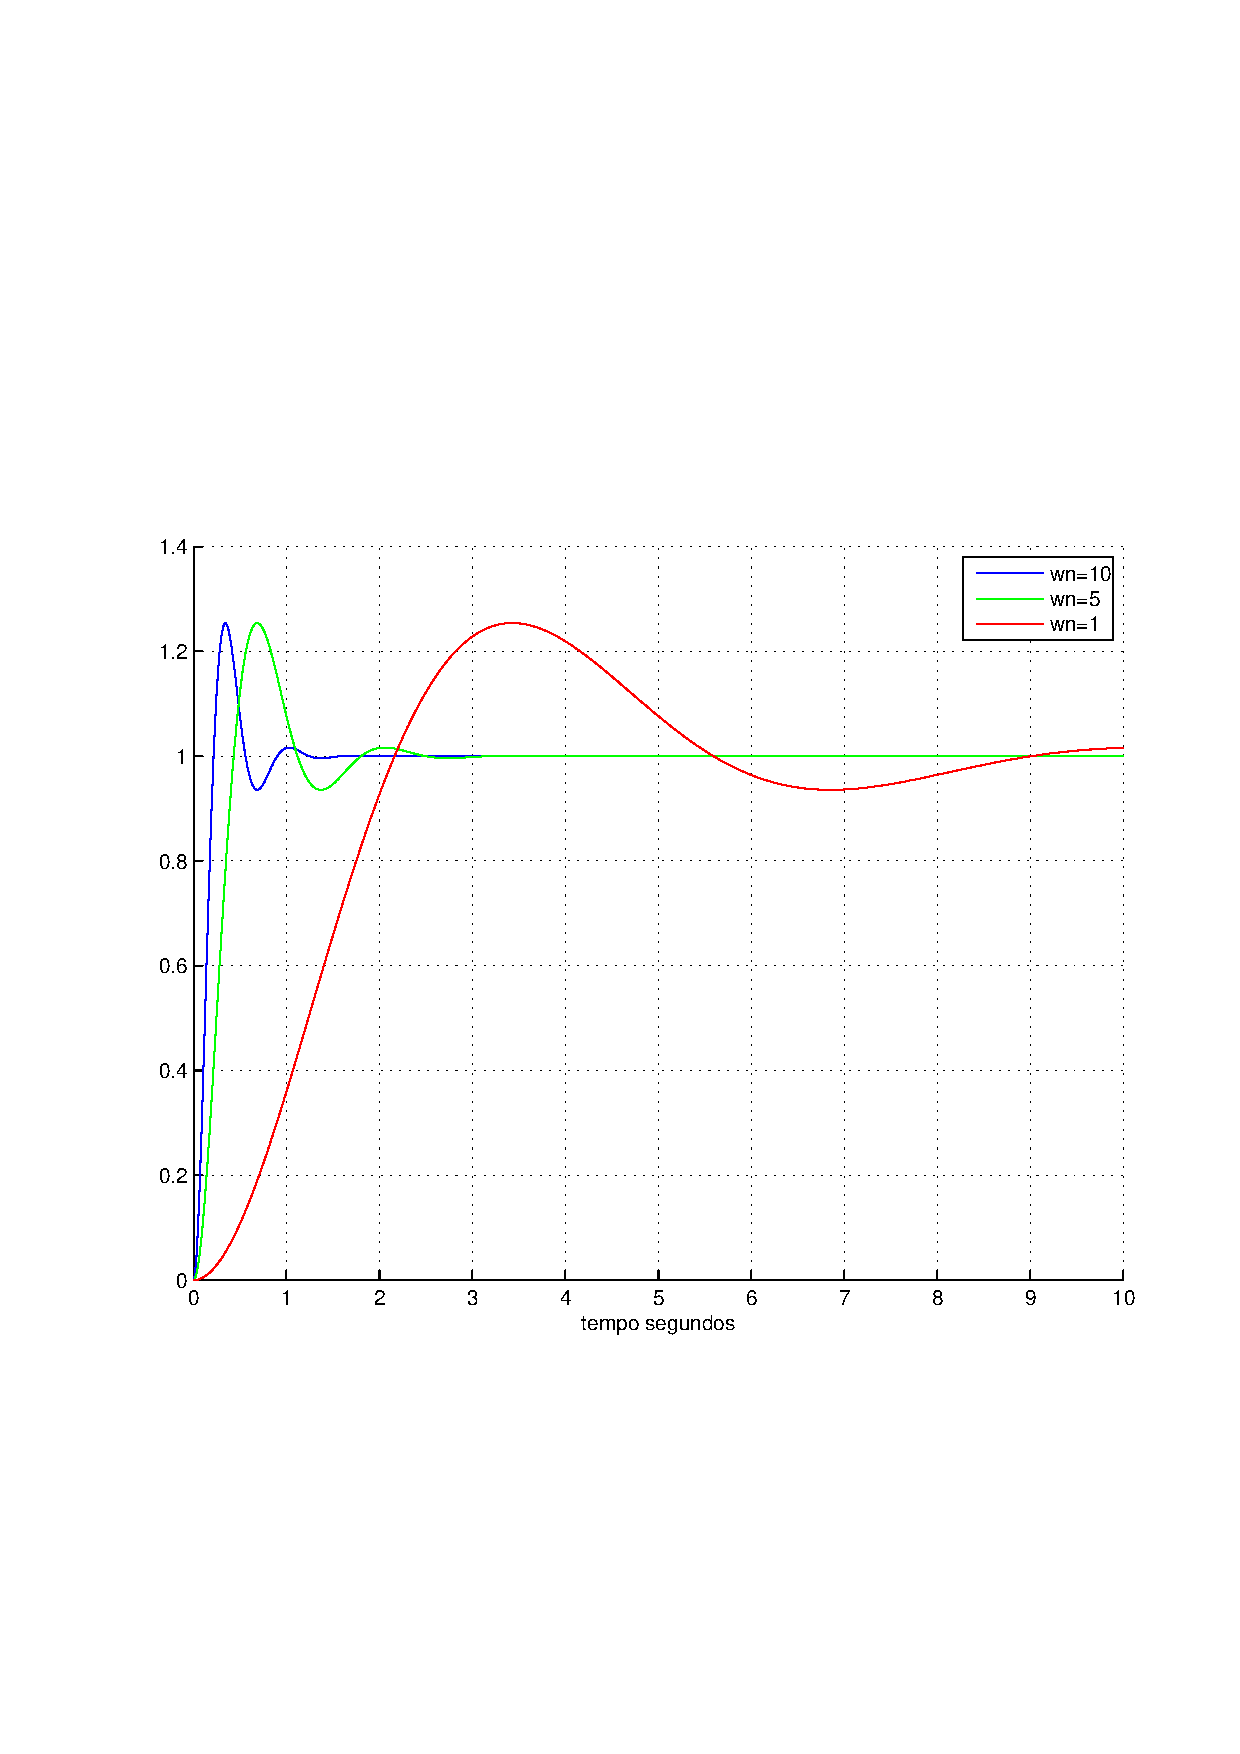
\includegraphics[scale=.5]{q1ia.pdf}
    \caption{Variações de $\omega_w$}
    \end{center}
\end{figure}

\subsection{Variação de $\zeta$}

Neste problema $\omega_n$ é fixo com valor de 5 e $\zeta$ assume os seguintes
valores: 0, 0.4, 0.6, 0.8, 1.0, 1.4.

Para tanto o mesmo código utilizado anteriormente para a analise de $\omega_n$
pode ser alterado para as variações de $\zeta$ de tal forma que fica,

\begin{lstlisting}
zeta = [0 0.4 0.6 0.8 1 1.4];
wn = 5;
t = 0:0.001:4;
cor = ['b', 'g', 'r', 'c', 'm', 'y'];
for c = 1:length(zeta)
    gs = tf([wn^2], [1 2*zeta(c)*wn wn^2]);
    [y(c,:)] = step(gs, t);
    hold on;
    plot(t, y(c,:), cor(c));
    grid on;
end
xlabel('tempo segundos');
\end{lstlisting}

A resposta para as diversas variações de $\zeta$ é apresentada na figura 2.

\begin{figure}
    \begin{center}
    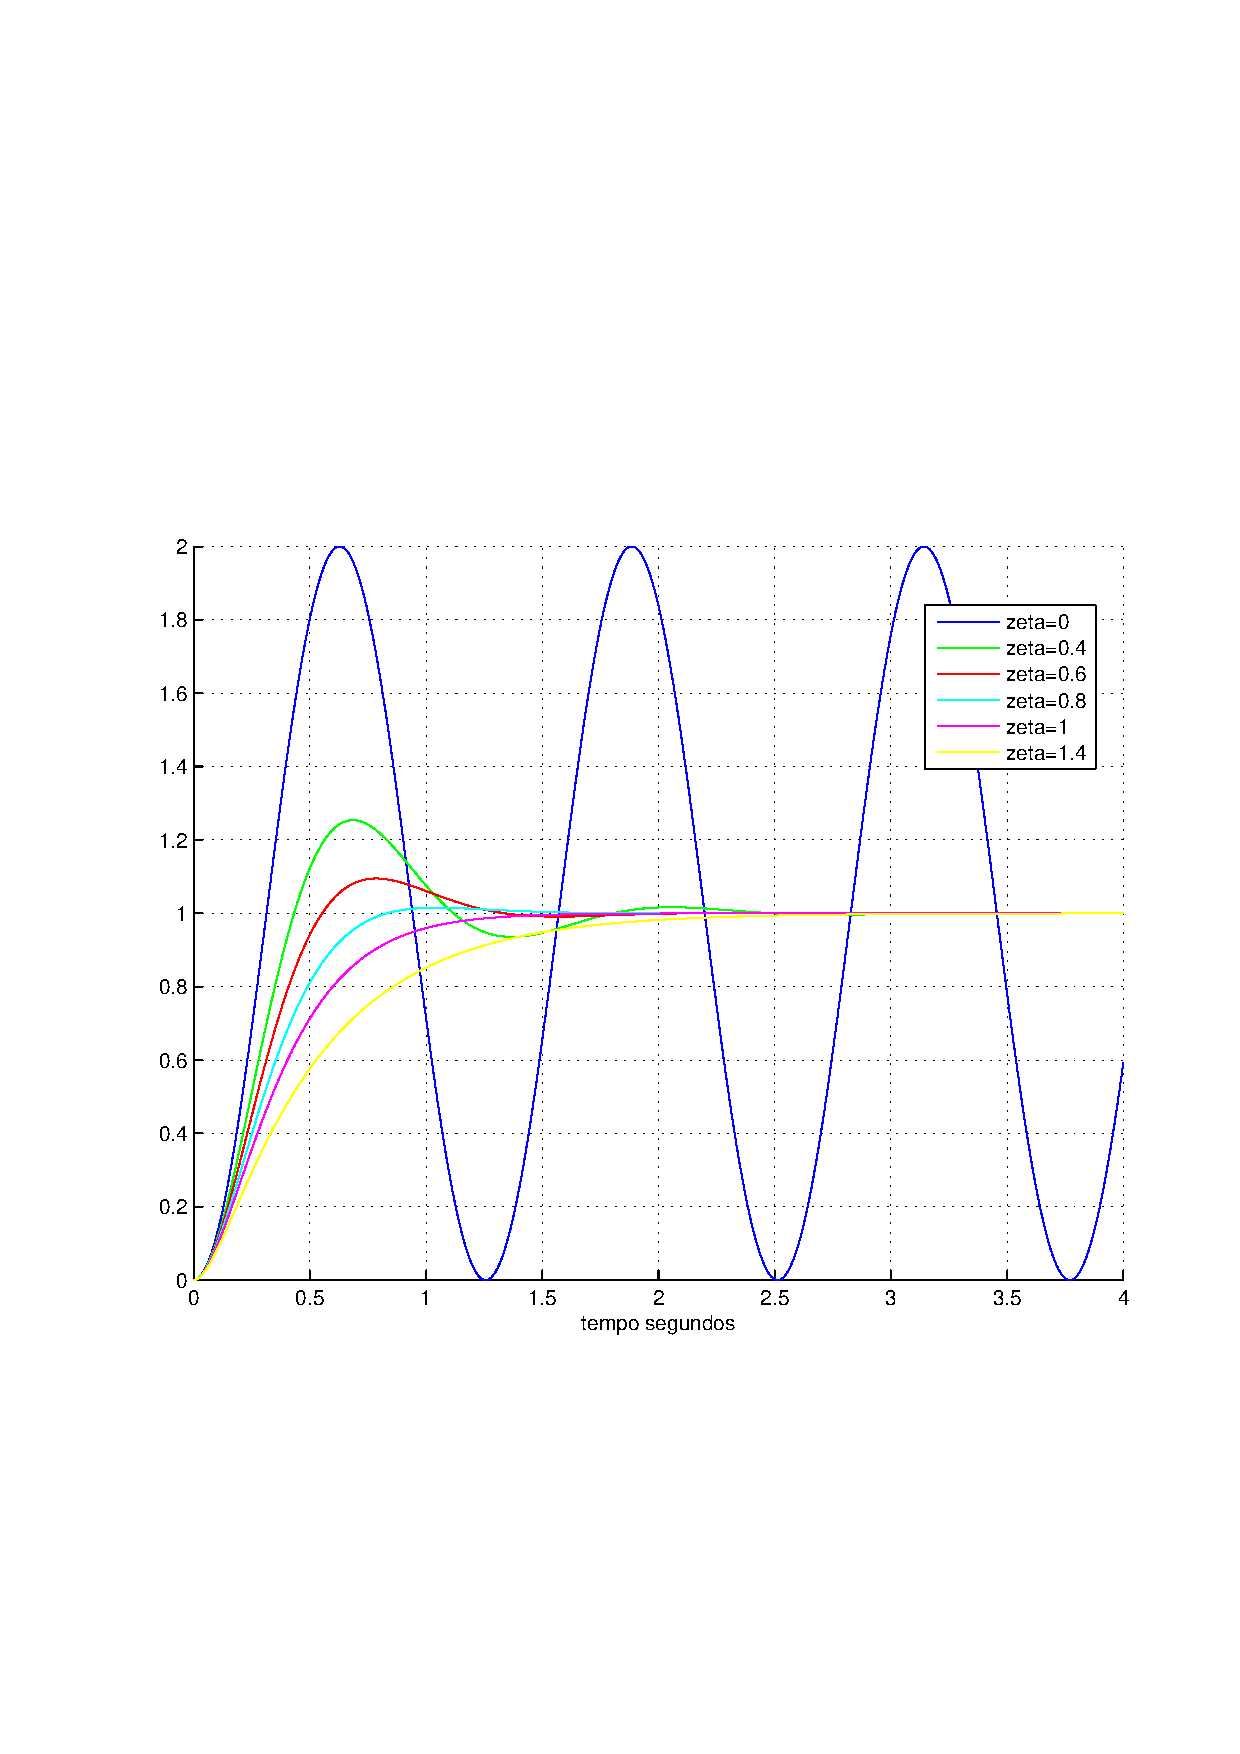
\includegraphics[scale=.5]{q1ib.pdf}
    \caption{Variações de $\zeta$}
    \end{center}
\end{figure}

\section{Grafico 3D}



\end{document}

